\chapter{Combinatorics}

\index{combinatorics}
\index{tổ hợp}

\key{Combinatorics} (Tổ hợp) nghiên cứu các phương pháp để đếm
các cách kết hợp các đối tượng.
Thông thường, mục tiêu là tìm cách
đếm các kết hợp một cách hiệu quả
mà không phải tạo ra từng kết hợp riêng lẻ.

Ví dụ, xét bài toán
đếm số cách
biểu diễn một số nguyên $n$ dưới dạng tổng các số nguyên dương.
Ví dụ, có 8 cách biểu diễn
cho $4$:
\begin{multicols}{2}
\begin{itemize}
\item $1+1+1+1$
\item $1+1+2$
\item $1+2+1$
\item $2+1+1$
\item $2+2$
\item $3+1$
\item $1+3$
\item $4$
\end{itemize}
\end{multicols}

Một bài toán tổ hợp thường có thể được giải
bằng cách sử dụng hàm đệ quy.
Trong bài toán này, chúng ta có thể định nghĩa một hàm $f(n)$
trả về số cách biểu diễn cho $n$.
Ví dụ, $f(4)=8$ theo ví dụ trên.
Các giá trị của hàm
có thể được tính đệ quy như sau:
\begin{equation*}
    f(n) = \begin{cases}
               1               & n = 0\\
               f(0)+f(1)+\cdots+f(n-1) & n > 0\\
           \end{cases}
\end{equation*}
Trường hợp cơ sở là $f(0)=1$,
bởi vì tổng rỗng biểu diễn số 0.
Sau đó, nếu $n>0$, ta xét tất cả các cách
chọn số đầu tiên của tổng.
Nếu số đầu tiên là $k$,
có $f(n-k)$ cách biểu diễn
cho phần còn lại của tổng.
Do đó, ta tính tổng của tất cả các giá trị
có dạng $f(n-k)$ với $k<n$.

Các giá trị đầu tiên của hàm là:
\[
\begin{array}{lcl}
f(0) & = & 1 \\
f(1) & = & 1 \\
f(2) & = & 2 \\
f(3) & = & 4 \\
f(4) & = & 8 \\
\end{array}
\]

Đôi khi, một công thức đệ quy có thể được thay thế
bằng một công thức dạng đóng (closed-form).
Trong bài toán này,
\[
f(n)=2^{n-1},
\]
dựa trên thực tế là có $n-1$
vị trí có thể đặt dấu + trong tổng
và ta có thể chọn bất kỳ tập con nào của chúng.

\section{Binomial coefficients}

\index{binomial coefficient}
\index{hệ số nhị thức}

The \key{binomial coefficient} (hệ số nhị thức) ${n \choose k}$
bằng số cách chọn một tập con
gồm $k$ phần tử từ một tập $n$ phần tử.
Ví dụ, ${5 \choose 3}=10$,
bởi vì tập $\{1,2,3,4,5\}$
có 10 tập con gồm 3 phần tử:
\[ \{1,2,3\}, \{1,2,4\}, \{1,2,5\}, \{1,3,4\}, \{1,3,5\}, 
\{1,4,5\}, \{2,3,4\}, \{2,3,5\}, \{2,4,5\}, \{3,4,5\} \]

\subsubsection{Formula 1}

Các hệ số nhị thức có thể được
tính đệ quy như sau:

\[
{n \choose k}  =  {n-1 \choose k-1} + {n-1 \choose k}
\]

Ý tưởng là cố định một phần tử $x$ trong tập.
Nếu $x$ được chọn vào tập con,
ta phải chọn $k-1$
phần tử từ $n-1$ phần tử còn lại,
và nếu $x$ không được chọn vào tập con,
ta phải chọn $k$ phần tử từ $n-1$ phần tử còn lại.

Các trường hợp cơ sở cho đệ quy là
\[
{n \choose 0}  =  {n \choose n} = 1,
\]
bởi vì luôn luôn chỉ có
một cách để tạo ra một tập con rỗng
và một tập con chứa tất cả các phần tử.

\subsubsection{Formula 2}

Một cách khác để tính hệ số nhị thức như sau:
\[
{n \choose k}  =  \frac{n!}{k!(n-k)!}.
\]

Có $n!$ hoán vị của $n$ phần tử.
Ta duyệt qua tất cả các hoán vị và luôn
chọn $k$ phần tử đầu tiên của hoán vị
vào tập con.
Vì thứ tự của các phần tử trong tập con
và ngoài tập con không quan trọng,
kết quả được chia cho $k!$ và $(n-k)!$

\subsubsection{Properties}

Đối với hệ số nhị thức,
\[
{n \choose k}  =  {n \choose n-k},
\]
bởi vì thực tế chúng ta chia một tập $n$ phần tử thành
hai tập con: tập thứ nhất chứa $k$ phần tử
và tập thứ hai chứa $n-k$ phần tử.

Tổng các hệ số nhị thức là
\[
{n \choose 0}+{n \choose 1}+{n \choose 2}+\ldots+{n \choose n}=2^n.
\]

Lý do cho tên gọi ''hệ số nhị thức''
có thể thấy khi nhị thức $(a+b)$ được lũy thừa
lên mũ thứ $n$:

\[ (a+b)^n =
{n \choose 0} a^n b^0 + 
{n \choose 1} a^{n-1} b^1 +
\ldots + 
{n \choose n-1} a^1 b^{n-1} +
{n \choose n} a^0 b^n. \]

\index{Pascal's triangle}
\index{tam giác Pascal}

Hệ số nhị thức cũng xuất hiện trong
\key{Pascal's triangle} (tam giác Pascal)
trong đó mỗi giá trị bằng tổng của hai
giá trị phía trên:
\begin{center}
\begin{tikzpicture}{0.9}
\node at (0,0) {1};
\node at (-0.5,-0.5) {1};
\node at (0.5,-0.5) {1};
\node at (-1,-1) {1};
\node at (0,-1) {2};
\node at (1,-1) {1};
\node at (-1.5,-1.5) {1};
\node at (-0.5,-1.5) {3};
\node at (0.5,-1.5) {3};
\node at (1.5,-1.5) {1};
\node at (-2,-2) {1};
\node at (-1,-2) {4};
\node at (0,-2) {6};
\node at (1,-2) {4};
\node at (2,-2) {1};
\node at (-2,-2.5) {$\ldots$};
\node at (-1,-2.5) {$\ldots$};
\node at (0,-2.5) {$\ldots$};
\node at (1,-2.5) {$\ldots$};
\node at (2,-2.5) {$\ldots$};
\end{tikzpicture}
\end{center}

\subsubsection{Boxes and balls}

''Boxes and balls'' (Hộp và bi) là một mô hình hữu ích,
trong đó ta đếm số cách để
đặt $k$ quả bi vào $n$ hộp.
Hãy xét ba kịch bản:

\textit{Scenario 1}: Mỗi hộp có thể chứa
tối đa một quả bi.
Ví dụ, khi $n=5$ và $k=2$,
có 10 cách giải:

\begin{center}
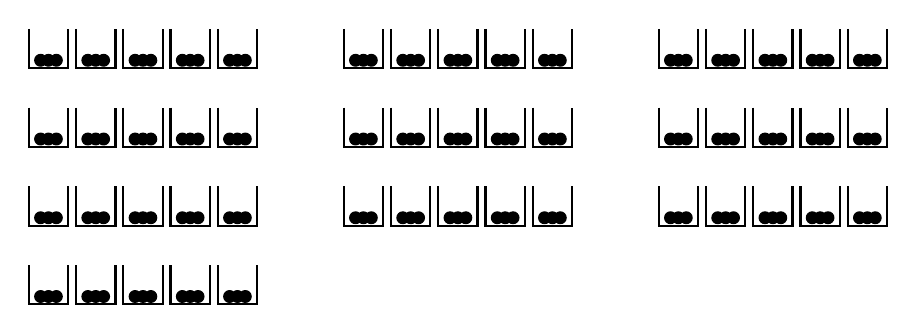
\begin{tikzpicture}[scale=0.5]
\newcommand\lax[3]{
\path[draw,thick,-] (#1-0.5,#2+0.5) -- (#1-0.5,#2-0.5) --
                    (#1+0.5,#2-0.5) -- (#1+0.5,#2+0.5);
\ifthenelse{\equal{#3}{1}}{\draw[fill=black] (#1,#2-0.3) circle (0.15);}{}
\ifthenelse{\equal{#3}{2}}{\draw[fill=black] (#1-0.2,#2-0.3) circle (0.15);}{}
\ifthenelse{\equal{#3}{2}}{\draw[fill=black] (#1+0.2,#2-0.3) circle (0.15);}{}
}
\newcommand\laa[7]{
    \lax{#1}{#2}{#3}
    \lax{#1+1.2}{#2}{#4}
    \lax{#1+2.4}{#2}{#5}
    \lax{#1+3.6}{#2}{#6}
    \lax{#1+4.8}{#2}{#7}
}

\laa{0}{0}{1}{1}{0}{0}{0}
\laa{0}{-2}{1}{0}{1}{0}{0}
\laa{0}{-4}{1}{0}{0}{1}{0}
\laa{0}{-6}{1}{0}{0}{0}{1}
\laa{8}{0}{0}{1}{1}{0}{0}
\laa{8}{-2}{0}{1}{0}{1}{0}
\laa{8}{-4}{0}{1}{0}{0}{1}
\laa{16}{0}{0}{0}{1}{1}{0}
\laa{16}{-2}{0}{0}{1}{0}{1}
\laa{16}{-4}{0}{0}{0}{1}{1}

\end{tikzpicture}
\end{center}

Trong kịch bản này, kết quả chính là
hệ số nhị thức ${n \choose k}$.

\textit{Scenario 2}: Một hộp có thể chứa nhiều quả bi.
Ví dụ, khi $n=5$ và $k=2$,
có 15 cách giải:

\begin{center}
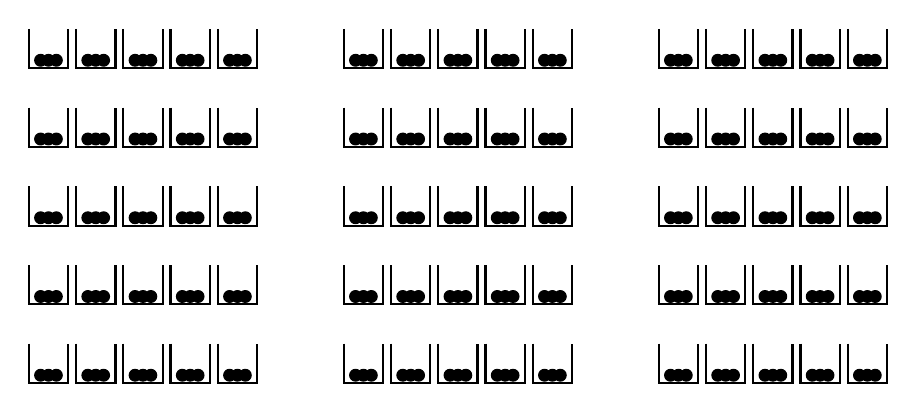
\begin{tikzpicture}[scale=0.5]
\newcommand\lax[3]{
\path[draw,thick,-] (#1-0.5,#2+0.5) -- (#1-0.5,#2-0.5) --
                    (#1+0.5,#2-0.5) -- (#1+0.5,#2+0.5);
\ifthenelse{\equal{#3}{1}}{\draw[fill=black] (#1,#2-0.3) circle (0.15);}{}
\ifthenelse{\equal{#3}{2}}{\draw[fill=black] (#1-0.2,#2-0.3) circle (0.15);}{}
\ifthenelse{\equal{#3}{2}}{\draw[fill=black] (#1+0.2,#2-0.3) circle (0.15);}{}
}
\newcommand\laa[7]{
    \lax{#1}{#2}{#3}
    \lax{#1+1.2}{#2}{#4}
    \lax{#1+2.4}{#2}{#5}
    \lax{#1+3.6}{#2}{#6}
    \lax{#1+4.8}{#2}{#7}
}

\laa{0}{0}{2}{0}{0}{0}{0}
\laa{0}{-2}{1}{1}{0}{0}{0}
\laa{0}{-4}{1}{0}{1}{0}{0}
\laa{0}{-6}{1}{0}{0}{1}{0}
\laa{0}{-8}{1}{0}{0}{0}{1}
\laa{8}{0}{0}{2}{0}{0}{0}
\laa{8}{-2}{0}{1}{1}{0}{0}
\laa{8}{-4}{0}{1}{0}{1}{0}
\laa{8}{-6}{0}{1}{0}{0}{1}
\laa{8}{-8}{0}{0}{2}{0}{0}
\laa{16}{0}{0}{0}{1}{1}{0}
\laa{16}{-2}{0}{0}{1}{0}{1}
\laa{16}{-4}{0}{0}{0}{2}{0}
\laa{16}{-6}{0}{0}{0}{1}{1}
\laa{16}{-8}{0}{0}{0}{0}{2}

\end{tikzpicture}
\end{center}

Quá trình đặt các quả bi vào các hộp
có thể được biểu diễn bằng một chuỗi
gồm các ký hiệu
''o'' và ''$\rightarrow$''.
Ban đầu, giả sử ta đang đứng ở hộp ngoài cùng bên trái.
Ký hiệu ''o'' có nghĩa là ta đặt một quả bi
vào hộp hiện tại, và ký hiệu
''$\rightarrow$'' có nghĩa là ta di chuyển đến
hộp tiếp theo bên phải.

Sử dụng ký hiệu này, mỗi cách giải là một chuỗi
chứa $k$ lần ký hiệu ''o'' và
$n-1$ lần ký hiệu ''$\rightarrow$''.
Ví dụ, cách giải ở góc trên bên phải
trong hình trên tương ứng với chuỗi
''$\rightarrow$ $\rightarrow$ o $\rightarrow$ o $\rightarrow$''.
Do đó, số cách giải là
${k+n-1 \choose k}$.

\textit{Scenario 3}: Mỗi hộp có thể chứa nhiều nhất một quả bi,
và thêm nữa, không có hai hộp liền kề nào đều chứa bi.
Ví dụ, khi $n=5$ và $k=2$,
có 6 cách giải:


\begin{center}
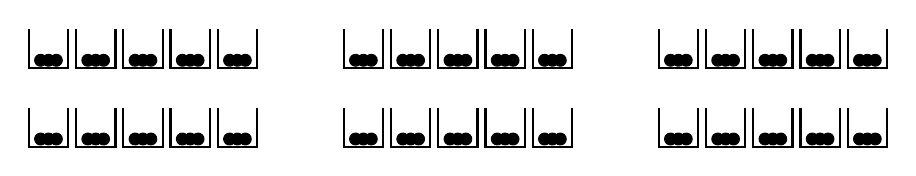
\begin{tikzpicture}[scale=0.5]
\newcommand\lax[3]{
\path[draw,thick,-] (#1-0.5,#2+0.5) -- (#1-0.5,#2-0.5) --
                    (#1+0.5,#2-0.5) -- (#1+0.5,#2+0.5);
\ifthenelse{\equal{#3}{1}}{\draw[fill=black] (#1,#2-0.3) circle (0.15);}{}
\ifthenelse{\equal{#3}{2}}{\draw[fill=black] (#1-0.2,#2-0.3) circle (0.15);}{}
\ifthenelse{\equal{#3}{2}}{\draw[fill=black] (#1+0.2,#2-0.3) circle (0.15);}{}
}
\newcommand\laa[7]{
    \lax{#1}{#2}{#3}
    \lax{#1+1.2}{#2}{#4}
    \lax{#1+2.4}{#2}{#5}
    \lax{#1+3.6}{#2}{#6}
    \lax{#1+4.8}{#2}{#7}
}

\laa{0}{0}{1}{0}{1}{0}{0}
\laa{0}{-2}{1}{0}{0}{1}{0}
\laa{8}{0}{1}{0}{0}{0}{1}
\laa{8}{-2}{0}{1}{0}{1}{0}
\laa{16}{0}{0}{1}{0}{0}{1}
\laa{16}{-2}{0}{0}{1}{0}{1}
\end{tikzpicture}
\end{center}

Trong kịch bản này, ta có thể giả sử rằng
$k$ quả bi được đặt vào các hộp ban đầu
và có một hộp trống giữa mỗi
cặp hộp liền kề.
Nhiệm vụ còn lại là chọn
vị trí cho các hộp trống còn lại.
Có $n-2k+1$ hộp như vậy và
$k+1$ vị trí cho chúng.
Do đó, sử dụng công thức của kịch bản 2,
số cách giải là
${n-k+1 \choose n-2k+1}$.

\subsubsection{Multinomial coefficients}

\index{multinomial coefficient}
\index{hệ số đa thức}

The \key{multinomial coefficient} (hệ số đa thức)
\[ {n \choose k_1,k_2,\ldots,k_m} = \frac{n!}{k_1! k_2! \cdots k_m!}, \]
bằng số cách
chúng ta có thể chia $n$ phần tử thành các tập con
có kích thước $k_1,k_2,\ldots,k_m$,
trong đó $k_1+k_2+\cdots+k_m=n$.
Hệ số đa thức có thể được xem như một
tổng quát hóa của hệ số nhị thức;
nếu $m=2$, công thức trên
tương ứng với công thức hệ số nhị thức.

\section{Catalan numbers}

\index{Catalan number}
\index{số Catalan}

The \key{Catalan number} (Số Catalan)
%\footnote{E. C. Catalan (1814--1894) was a Belgian mathematician.}
$C_n$ bằng
số biểu thức dấu ngoặc hợp lệ
gồm $n$ dấu ngoặc trái và $n$ dấu ngoặc phải.

Ví dụ, $C_3=5$, bởi vì
chúng ta có thể tạo ra các biểu thức
dấu ngoặc sau sử dụng ba
dấu ngoặc trái và phải:

\begin{itemize}[noitemsep]
\item \texttt{()()()}
\item \texttt{(())()}
\item \texttt{()(())}
\item \texttt{((()))}
\item \texttt{(()())}
\end{itemize}

\subsubsection{Parenthesis expressions}

\index{parenthesis expression}
\index{biểu thức dấu ngoặc}

\emph{Biểu thức dấu ngoặc hợp lệ} là gì?
Các quy tắc sau xác định chính xác tất cả
biểu thức dấu ngoặc hợp lệ:

\begin{itemize}
\item Biểu thức dấu ngoặc rỗng là hợp lệ.
\item Nếu biểu thức $A$ hợp lệ,
thì biểu thức
\texttt{(}$A$\texttt{)} cũng hợp lệ.
\item Nếu biểu thức $A$ và $B$ hợp lệ,
thì biểu thức $AB$ cũng hợp lệ.
\end{itemize}

Một cách khác để mô tả biểu thức
dấu ngoặc hợp lệ là nếu
chúng ta chọn bất kỳ tiền tố nào của biểu thức đó,
nó phải chứa ít nhất bằng nhiều dấu ngoặc
trái như dấu ngoặc phải.
Ngoài ra, biểu thức hoàn chỉnh phải
chứa số lượng dấu ngoặc trái và phải bằng nhau.

\subsubsection{Formula 1}

Số Catalan có thể được tính bằng công thức
\[ C_n = \sum_{i=0}^{n-1} C_{i} C_{n-i-1}.\]

Tổng này duyệt qua các cách để chia
biểu thức thành hai phần
sao cho cả hai phần đều là các biểu thức
hợp lệ và phần đầu tiên ngắn nhất có thể
nhưng không rỗng.
Với mọi $i$, phần đầu tiên chứa $i+1$ cặp
dấu ngoặc và số lượng biểu thức
là tích của các giá trị sau:

\begin{itemize}
\item $C_{i}$: số cách để tạo một biểu thức
sử dụng các dấu ngoặc của phần đầu tiên,
không tính cặp ngoặc ngoài cùng
\item $C_{n-i-1}$: số cách để tạo một
biểu thức sử dụng các dấu ngoặc của phần thứ hai
\end{itemize}

Trường hợp cơ sở là $C_0=1$,
bởi vì ta có thể tạo một biểu thức
dấu ngoặc rỗng sử dụng không cặp dấu ngoặc nào.

\subsubsection{Formula 2}

Số Catalan cũng có thể được tính
sử dụng hệ số nhị thức:
\[ C_n = \frac{1}{n+1} {2n \choose n}\]
Công thức có thể được giải thích như sau:

Có tổng cộng ${2n \choose n}$ cách
để tạo một biểu thức dấu ngoặc (không nhất thiết hợp lệ)
chứa $n$ dấu ngoặc trái và
$n$ dấu ngoặc phải.
Hãy tính số lượng biểu thức như vậy
mà \emph{không} hợp lệ.

Nếu một biểu thức dấu ngoặc không hợp lệ,
nó phải chứa một tiền tố trong đó
số dấu ngoặc phải nhiều hơn
số dấu ngoặc trái.
Ý tưởng là đảo ngược mỗi dấu ngoặc
thuộc tiền tố đó.
Ví dụ, biểu thức
\texttt{())()(} chứa tiền tố \texttt{())},
và sau khi đảo ngược tiền tố,
biểu thức trở thành \texttt{)((()(}.

Biểu thức kết quả gồm $n+1$
dấu ngoặc trái và $n-1$ dấu ngoặc phải.
Số lượng biểu thức như vậy là ${2n \choose n+1}$,
bằng số lượng biểu thức dấu ngoặc
không hợp lệ.
Do đó, số lượng biểu thức dấu ngoặc
hợp lệ có thể được tính bằng công thức
\[{2n \choose n}-{2n \choose n+1} = {2n \choose n} - \frac{n}{n+1} {2n \choose n} = \frac{1}{n+1} {2n \choose n}.\]

\subsubsection{Counting trees}

Số Catalan cũng liên quan đến cây:

\begin{itemize}
\item có $C_n$ cây nhị phân với $n$ nút
\item có $C_{n-1}$ cây có gốc với $n$ nút
\end{itemize}
\noindent
Ví dụ, với $C_3=5$, các cây nhị phân là

\begin{center}
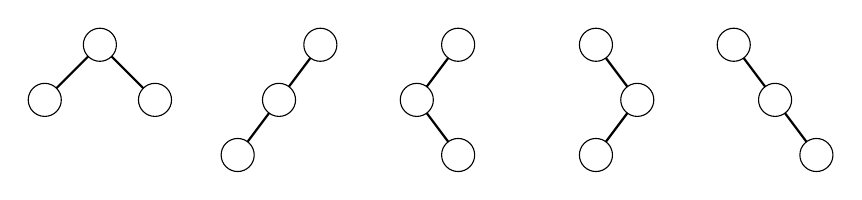
\begin{tikzpicture}[scale=0.7]
\path[draw,thick,-] (0,0) -- (-1,-1);
\path[draw,thick,-] (0,0) -- (1,-1);
\draw[fill=white] (0,0) circle (0.3);
\draw[fill=white] (-1,-1) circle (0.3);
\draw[fill=white] (1,-1) circle (0.3);

\path[draw,thick,-] (4,0) -- (4-0.75,-1) -- (4-1.5,-2);
\draw[fill=white] (4,0) circle (0.3);
\draw[fill=white] (4-0.75,-1) circle (0.3);
\draw[fill=white] (4-1.5,-2) circle (0.3);

\path[draw,thick,-] (6.5,0) -- (6.5-0.75,-1) -- (6.5-0,-2);
\draw[fill=white] (6.5,0) circle (0.3);
\draw[fill=white] (6.5-0.75,-1) circle (0.3);
\draw[fill=white] (6.5-0,-2) circle (0.3);

\path[draw,thick,-] (9,0) -- (9+0.75,-1) -- (9-0,-2);
\draw[fill=white] (9,0) circle (0.3);
\draw[fill=white] (9+0.75,-1) circle (0.3);
\draw[fill=white] (9-0,-2) circle (0.3);

\path[draw,thick,-] (11.5,0) -- (11.5+0.75,-1) -- (11.5+1.5,-2);
\draw[fill=white] (11.5,0) circle (0.3);
\draw[fill=white] (11.5+0.75,-1) circle (0.3);
\draw[fill=white] (11.5+1.5,-2) circle (0.3);
\end{tikzpicture}
\end{center}
and the rooted trees are
\begin{center}
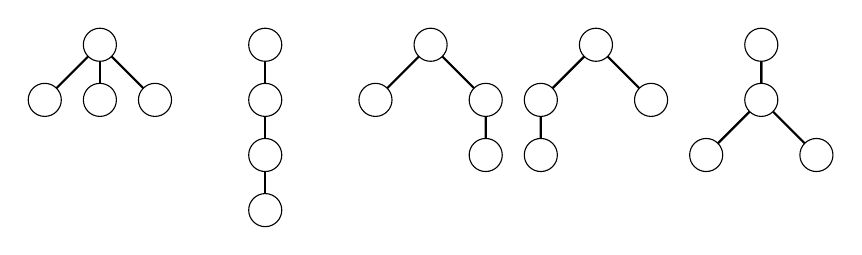
\begin{tikzpicture}[scale=0.7]
\path[draw,thick,-] (0,0) -- (-1,-1);
\path[draw,thick,-] (0,0) -- (0,-1);
\path[draw,thick,-] (0,0) -- (1,-1);
\draw[fill=white] (0,0) circle (0.3);
\draw[fill=white] (-1,-1) circle (0.3);
\draw[fill=white] (0,-1) circle (0.3);
\draw[fill=white] (1,-1) circle (0.3);

\path[draw,thick,-] (3,0) -- (3,-1) -- (3,-2) -- (3,-3);
\draw[fill=white] (3,0) circle (0.3);
\draw[fill=white] (3,-1) circle (0.3);
\draw[fill=white] (3,-2) circle (0.3);
\draw[fill=white] (3,-3) circle (0.3);

\path[draw,thick,-] (6+0,0) -- (6-1,-1);
\path[draw,thick,-] (6+0,0) -- (6+1,-1) -- (6+1,-2);
\draw[fill=white] (6+0,0) circle (0.3);
\draw[fill=white] (6-1,-1) circle (0.3);
\draw[fill=white] (6+1,-1) circle (0.3);
\draw[fill=white] (6+1,-2) circle (0.3);

\path[draw,thick,-] (9+0,0) -- (9+1,-1);
\path[draw,thick,-] (9+0,0) -- (9-1,-1) -- (9-1,-2);
\draw[fill=white] (9+0,0) circle (0.3);
\draw[fill=white] (9+1,-1) circle (0.3);
\draw[fill=white] (9-1,-1) circle (0.3);
\draw[fill=white] (9-1,-2) circle (0.3);

\path[draw,thick,-] (12+0,0) -- (12+0,-1) -- (12-1,-2);
\path[draw,thick,-] (12+0,0) -- (12+0,-1) -- (12+1,-2);
\draw[fill=white] (12+0,0) circle (0.3);
\draw[fill=white] (12+0,-1) circle (0.3);
\draw[fill=white] (12-1,-2) circle (0.3);
\draw[fill=white] (12+1,-2) circle (0.3);

\end{tikzpicture}
\end{center}

\section{Inclusion-exclusion}

\index{inclusion-exclusion}
\index{nguyên lý bao hàm-loại trừ}

\key{Inclusion-exclusion} (Nguyên lý bao hàm-loại trừ) là một kỹ thuật
có thể được sử dụng để đếm kích thước
của hợp các tập khi kích thước của
các giao đã biết, và ngược lại.
Một ví dụ đơn giản của kỹ thuật này là công thức
\[ |A \cup B| = |A| + |B| - |A \cap B|,\]
trong đó $A$ và $B$ là các tập và $|X|$
ký hiệu kích thước của $X$.
Công thức có thể được minh họa như sau:

\begin{center}
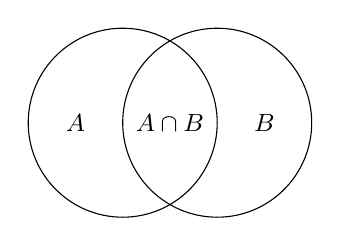
\begin{tikzpicture}[scale=0.8]

\draw (0,0) circle (1.5);
\draw (1.5,0) circle (1.5);

\node at (-0.75,0) {\small $A$};
\node at (2.25,0) {\small $B$};
\node at (0.75,0) {\small $A \cap B$};

\end{tikzpicture}
\end{center}

Mục tiêu của chúng ta là tính
kích thước của hợp $A \cup B$
tương ứng với diện tích của vùng
thuộc ít nhất một vòng tròn.
Hình vẽ cho thấy chúng ta có thể tính
diện tích của $A \cup B$ bằng cách đầu tiên cộng
diện tích của $A$ và $B$ và sau đó trừ đi
diện tích của $A \cap B$.

Cùng một ý tưởng có thể áp dụng khi số lượng
tập hợp lớn hơn.
Khi có ba tập, công thức bao hàm-loại trừ là
\[ |A \cup B \cup C| = |A| + |B| + |C| - |A \cap B|  - |A \cap C|  - |B \cap C| + |A \cap B \cap C| \]
và hình vẽ tương ứng là

\begin{center}
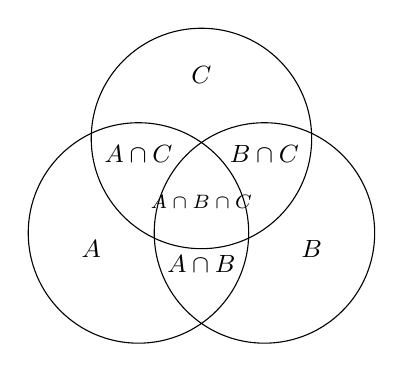
\begin{tikzpicture}[scale=0.8]

\draw (0,0) circle (1.75);
\draw (2,0) circle (1.75);
\draw (1,1.5) circle (1.75);

\node at (-0.75,-0.25) {\small $A$};
\node at (2.75,-0.25) {\small $B$};
\node at (1,2.5) {\small $C$};
\node at (1,-0.5) {\small $A \cap B$};
\node at (0,1.25) {\small $A \cap C$};
\node at (2,1.25) {\small $B \cap C$};
\node at (1,0.5) {\scriptsize $A \cap B \cap C$};

\end{tikzpicture}
\end{center}

Trong trường hợp tổng quát, kích thước của 
hợp $X_1 \cup X_2 \cup \cdots \cup X_n$
có thể được tính bằng cách xét tất cả các
giao có thể chứa một số tập trong $X_1,X_2,\ldots,X_n$.
Nếu giao chứa một số lẻ tập,
kích thước của nó được cộng vào kết quả,
và ngược lại kích thước của nó được trừ khỏi kết quả.

Chú ý rằng có những công thức tương tự
để tính
kích thước của giao từ kích thước của
các hợp. Ví dụ,
\[ |A \cap B| = |A| + |B| - |A \cup B|\]
và
\[ |A \cap B \cap C| = |A| + |B| + |C| - |A \cup B|  - |A \cup C|  - |B \cup C| + |A \cup B \cup C| .\]

\subsubsection{Derangements}

\index{derangement}
\index{hoán vị tráo trộn}

Để ví dụ, hãy đếm số \key{derangements} (hoán vị tráo trộn)
của các phần tử $\{1,2,\ldots,n\}$, tức là các hoán vị
trong đó không có phần tử nào giữ vị trí ban đầu của nó.
Ví dụ, khi $n=3$, có
hai hoán vị tráo trộn: $(2,3,1)$ và $(3,1,2)$.

Một cách tiếp cận để giải bài toán là sử dụng
nguyên lý bao hàm-loại trừ.
Gọi $X_k$ là tập các hoán vị
chứa phần tử $k$ tại vị trí $k$.
Ví dụ, khi $n=3$, các tập như sau:
\[
\begin{array}{lcl}
X_1 & = & \{(1,2,3),(1,3,2)\} \\
X_2 & = & \{(1,2,3),(3,2,1)\} \\
X_3 & = & \{(1,2,3),(2,1,3)\} \\
\end{array}
\]
Sử dụng các tập này, số hoán vị tráo trộn bằng
\[ n! - |X_1 \cup X_2 \cup \cdots \cup X_n|, \]
vậy chỉ cần tính kích thước của hợp.
Sử dụng nguyên lý bao hàm-loại trừ, điều này quy về
việc tính kích thước của các giao có thể được
thực hiện hiệu quả.
Ví dụ, khi $n=3$, kích thước của
$|X_1 \cup X_2 \cup X_3|$ là
\[
\begin{array}{lcl}
 & & |X_1| + |X_2| + |X_3| - |X_1 \cap X_2|  - |X_1 \cap X_3|  - |X_2 \cap X_3| + |X_1 \cap X_2 \cap X_3| \\
 & = & 2+2+2-1-1-1+1 \\
 & = & 4, \\
\end{array}
\]
vậy số nghiệm là $3!-4=2$.

Hóa ra bài toán cũng có thể được giải
mà không cần sử dụng nguyên lý bao hàm-loại trừ.
Gọi $f(n)$ là số hoán vị tráo trộn
cho $\{1,2,\ldots,n\}$. Ta có thể sử dụng
công thức đệ quy sau:

\begin{equation*}
    f(n) = \begin{cases}
               0               & n = 1\\
               1               & n = 2\\
               (n-1)(f(n-2) + f(n-1)) & n>2 \\
           \end{cases}
\end{equation*}

Công thức có thể được suy ra bằng cách xét
các khả năng phần tử 1 thay đổi
trong hoán vị tráo trộn.
Có $n-1$ cách để chọn một phần tử $x$
thay thế cho phần tử 1.
Trong mỗi lựa chọn như vậy, có hai phương án:

\textit{Option 1:} Ta cũng thay thế phần tử $x$
bằng phần tử 1.
Sau đó, nhiệm vụ còn lại là xây dựng
một hoán vị tráo trộn của $n-2$ phần tử.

\textit{Option 2:} Ta thay thế phần tử $x$
bằng một phần tử khác 1.
Bây giờ ta phải xây dựng một hoán vị tráo trộn
của $n-1$ phần tử, bởi vì ta không thể thay thế
phần tử $x$ bằng phần tử $1$, và tất cả các phần tử khác
phải được thay đổi.

\section{Burnside's lemma}

\index{Burnside's lemma}
\index{bổ đề Burnside}

\key{Burnside's lemma} (Bổ đề Burnside)
%\footnote{Actually, Burnside did not discover this lemma; he only mentioned it in his book \cite{bur97}.}
có thể được sử dụng để đếm
số lượng tổ hợp sao cho
chỉ đếm một đại diện
cho mỗi nhóm các tổ hợp đối xứng.
Bổ đề Burnside phát biểu rằng số lượng
tổ hợp là
\[\sum_{k=1}^n \frac{c(k)}{n},\]
trong đó có $n$ cách để thay đổi
vị trí của một tổ hợp,
và có $c(k)$ tổ hợp
không thay đổi khi áp dụng cách thứ $k$.

Để ví dụ, hãy tính số lượng
vòng cổ gồm $n$ hạt ngọc,
trong đó mỗi hạt ngọc có $m$ màu có thể.
Hai vòng cổ được gọi là đối xứng nếu chúng
giống nhau sau khi xoay.
For example, the necklace
\begin{center}
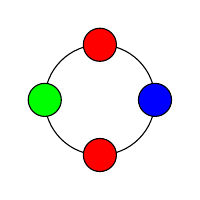
\begin{tikzpicture}[scale=0.7]
\draw[fill=white] (0,0) circle (1);
\draw[fill=red] (0,1) circle (0.3);
\draw[fill=blue] (1,0) circle (0.3);
\draw[fill=red] (0,-1) circle (0.3);
\draw[fill=green] (-1,0) circle (0.3);
\end{tikzpicture}
\end{center}
has the following symmetric necklaces:
\begin{center}
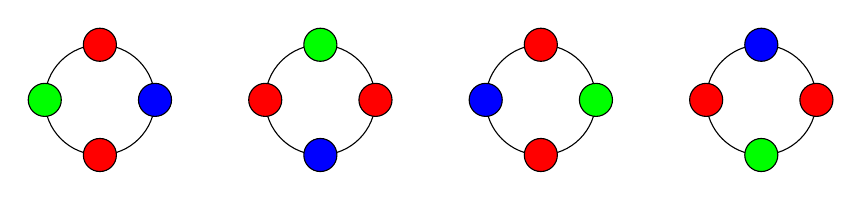
\begin{tikzpicture}[scale=0.7]
\draw[fill=white] (0,0) circle (1);
\draw[fill=red] (0,1) circle (0.3);
\draw[fill=blue] (1,0) circle (0.3);
\draw[fill=red] (0,-1) circle (0.3);
\draw[fill=green] (-1,0) circle (0.3);

\draw[fill=white] (4,0) circle (1);
\draw[fill=green] (4+0,1) circle (0.3);
\draw[fill=red] (4+1,0) circle (0.3);
\draw[fill=blue] (4+0,-1) circle (0.3);
\draw[fill=red] (4+-1,0) circle (0.3);

\draw[fill=white] (8,0) circle (1);
\draw[fill=red] (8+0,1) circle (0.3);
\draw[fill=green] (8+1,0) circle (0.3);
\draw[fill=red] (8+0,-1) circle (0.3);
\draw[fill=blue] (8+-1,0) circle (0.3);

\draw[fill=white] (12,0) circle (1);
\draw[fill=blue] (12+0,1) circle (0.3);
\draw[fill=red] (12+1,0) circle (0.3);
\draw[fill=green] (12+0,-1) circle (0.3);
\draw[fill=red] (12+-1,0) circle (0.3);
\end{tikzpicture}
\end{center}
Có $n$ cách để thay đổi vị trí
của một vòng cổ,
bởi vì ta có thể xoay nó
$0,1,\ldots,n-1$ bước theo chiều kim đồng hồ.
Nếu số bước là 0,
tất cả $m^n$ vòng cổ vẫn giữ nguyên,
và nếu số bước là 1,
chỉ có $m$ vòng cổ mà mỗi
hạt ngọc có cùng màu vẫn giữ nguyên.

Tổng quát hơn, khi số bước là $k$,
tổng cộng
\[m^{\textrm{gcd}(k,n)}\]
vòng cổ vẫn giữ nguyên,
trong đó $\textrm{gcd}(k,n)$ là ước số chung
lớn nhất của $k$ và $n$.
Lý do là các khối
hạt ngọc có kích thước $\textrm{gcd}(k,n)$
sẽ thay thế lẫn nhau.
Do đó, theo bổ đề Burnside,
số lượng vòng cổ là
\[\sum_{i=0}^{n-1} \frac{m^{\textrm{gcd}(i,n)}}{n}. \]
Ví dụ, số lượng vòng cổ độ dài 4
với 3 màu là
\[\frac{3^4+3+3^2+3}{4} = 24. \]

\section{Cayley's formula}

\index{Cayley's formula}
\index{công thức Cayley}

\key{Cayley's formula} (Công thức Cayley)
% \footnote{While the formula is named after A. Cayley,
% who studied it in 1889, it was discovered earlier by C. W. Borchardt in 1860.}
phát biểu rằng
có $n^{n-2}$ cây có gán nhãn
chứa $n$ nút.
Các nút được gán nhãn $1,2,\ldots,n$,
và hai cây được coi là khác nhau
nếu cấu trúc hoặc
cách gán nhãn của chúng khác nhau.

\begin{samepage}
Ví dụ, khi $n=4$, số lượng cây có gán nhãn
là $4^{4-2}=16$:

\begin{center}
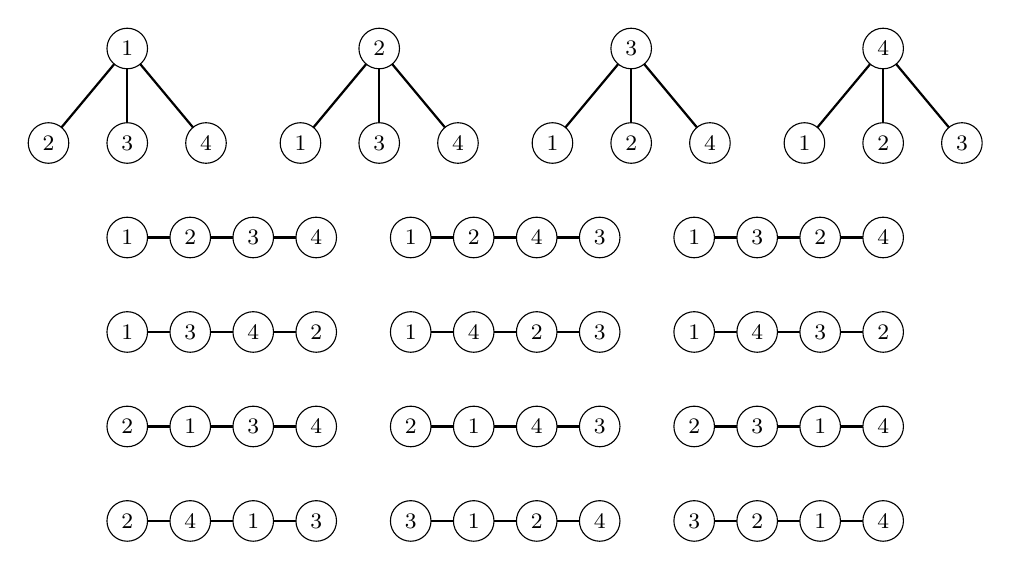
\begin{tikzpicture}[scale=0.8]
\footnotesize

\newcommand\puua[6]{
\path[draw,thick,-] (#1,#2) -- (#1-1.25,#2-1.5);
\path[draw,thick,-] (#1,#2) -- (#1,#2-1.5);
\path[draw,thick,-] (#1,#2) -- (#1+1.25,#2-1.5);
\node[draw, circle, fill=white] at (#1,#2) {#3};
\node[draw, circle, fill=white] at (#1-1.25,#2-1.5) {#4};
\node[draw, circle, fill=white] at (#1,#2-1.5) {#5};
\node[draw, circle, fill=white] at (#1+1.25,#2-1.5) {#6};
}
\newcommand\puub[6]{
\path[draw,thick,-] (#1,#2) -- (#1+1,#2);
\path[draw,thick,-] (#1+1,#2) -- (#1+2,#2);
\path[draw,thick,-] (#1+2,#2) -- (#1+3,#2);
\node[draw, circle, fill=white] at (#1,#2) {#3};
\node[draw, circle, fill=white] at (#1+1,#2) {#4};
\node[draw, circle, fill=white] at (#1+2,#2) {#5};
\node[draw, circle, fill=white] at (#1+3,#2) {#6};
}

\puua{0}{0}{1}{2}{3}{4}
\puua{4}{0}{2}{1}{3}{4}
\puua{8}{0}{3}{1}{2}{4}
\puua{12}{0}{4}{1}{2}{3}

\puub{0}{-3}{1}{2}{3}{4}
\puub{4.5}{-3}{1}{2}{4}{3}
\puub{9}{-3}{1}{3}{2}{4}
\puub{0}{-4.5}{1}{3}{4}{2}
\puub{4.5}{-4.5}{1}{4}{2}{3}
\puub{9}{-4.5}{1}{4}{3}{2}
\puub{0}{-6}{2}{1}{3}{4}
\puub{4.5}{-6}{2}{1}{4}{3}
\puub{9}{-6}{2}{3}{1}{4}
\puub{0}{-7.5}{2}{4}{1}{3}
\puub{4.5}{-7.5}{3}{1}{2}{4}
\puub{9}{-7.5}{3}{2}{1}{4}
\end{tikzpicture}
\end{center}
\end{samepage}

Tiếp theo chúng ta sẽ thấy cách chứng minh công thức Cayley
bằng cách sử dụng mã Prüfer (Prüfer codes).

\subsubsection{Mã Prüfer}

\index{Prüfer code}
\index{mã Prüfer}

\key{Mã Prüfer} (Prüfer code)
%\footnote{In 1918, H. Prüfer proved Cayley's theorem using Prüfer codes \cite{pru18}.}
là một dãy gồm
$n-2$ số mô tả một cây có gán nhãn.
Mã này được tạo ra bằng cách thực hiện một quá trình
loại bỏ $n-2$ lá khỏi cây.
Ở mỗi bước, lá có nhãn nhỏ nhất sẽ bị loại bỏ,
và nhãn của nút kề duy nhất của nó được thêm vào mã.

Ví dụ, hãy tính mã Prüfer
của đồ thị sau:
\begin{center}
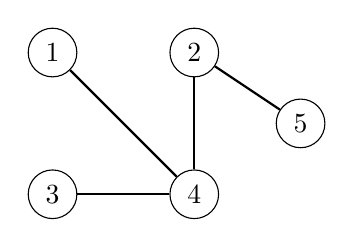
\begin{tikzpicture}[scale=0.9]
\node[draw, circle] (1) at (2,3) {$1$};
\node[draw, circle] (2) at (4,3) {$2$};
\node[draw, circle] (3) at (2,1) {$3$};
\node[draw, circle] (4) at (4,1) {$4$};
\node[draw, circle] (5) at (5.5,2) {$5$};

\path[draw,thick,-] (1) -- (4);
\path[draw,thick,-] (3) -- (4);
\path[draw,thick,-] (2) -- (4);
\path[draw,thick,-] (2) -- (5);
\end{tikzpicture}
\end{center}

Đầu tiên ta loại bỏ nút 1 và thêm nút 4 vào mã:
\begin{center}
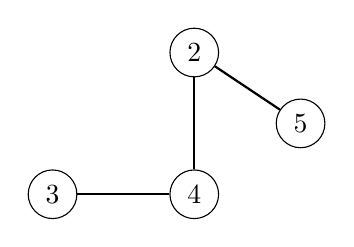
\begin{tikzpicture}[scale=0.9]
%\node[draw, circle] (1) at (2,3) {$1$};
\node[draw, circle] (2) at (4,3) {$2$};
\node[draw, circle] (3) at (2,1) {$3$};
\node[draw, circle] (4) at (4,1) {$4$};
\node[draw, circle] (5) at (5.5,2) {$5$};

%\path[draw,thick,-] (1) -- (4);
\path[draw,thick,-] (3) -- (4);
\path[draw,thick,-] (2) -- (4);
\path[draw,thick,-] (2) -- (5);
\end{tikzpicture}
\end{center}

Sau đó ta loại bỏ nút 3 và thêm nút 4 vào mã:
\begin{center}
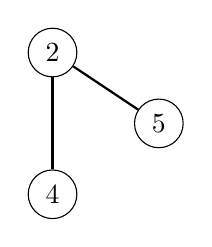
\begin{tikzpicture}[scale=0.9]
%\node[draw, circle] (1) at (2,3) {$1$};
\node[draw, circle] (2) at (4,3) {$2$};
%\node[draw, circle] (3) at (2,1) {$3$};
\node[draw, circle] (4) at (4,1) {$4$};
\node[draw, circle] (5) at (5.5,2) {$5$};

%\path[draw,thick,-] (1) -- (4);
%\path[draw,thick,-] (3) -- (4);
\path[draw,thick,-] (2) -- (4);
\path[draw,thick,-] (2) -- (5);
\end{tikzpicture}
\end{center}

Cuối cùng ta loại bỏ nút 4 và thêm nút 2 vào mã:
\begin{center}
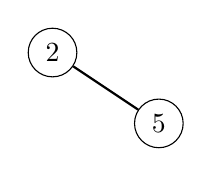
\begin{tikzpicture}[scale=0.9]
%\node[draw, circle] (1) at (2,3) {$1$};
\node[draw, circle] (2) at (4,3) {$2$};
%\node[draw, circle] (3) at (2,1) {$3$};
%\node[draw, circle] (4) at (4,1) {$4$};
\node[draw, circle] (5) at (5.5,2) {$5$};

%\path[draw,thick,-] (1) -- (4);
%\path[draw,thick,-] (3) -- (4);
%\path[draw,thick,-] (2) -- (4);
\path[draw,thick,-] (2) -- (5);
\end{tikzpicture}
\end{center}

Vậy mã Prüfer của đồ thị là $[4,4,2]$.

Ta có thể xây dựng một mã Prüfer cho bất kỳ cây nào,
và quan trọng hơn,
cây ban đầu có thể được tái tạo lại
từ một mã Prüfer.
Do đó, số lượng cây gán nhãn
có $n$ nút bằng
$n^{n-2}$, số lượng mã Prüfer
có kích thước $n$.
